\chapter{Classification}
Classification is a form of supervised machine learning (in contrary to Clustering, see chapter \ref{chap:clustering}. It takes examples which we have identified with classes and tries to learn a model that will predict the class of unknown examples. An example of use is to classify tumors as benign or malignant. We feed the classifier the features, such as size and shape, of known results. After the learning phase we can then use this classifier to predict if a given tumor is benign or not.

\section{K Nearest Neighbors}
KNN is a simple but effective classification algorithm. The algorithm works by finding the k neirest neighbors of a given data point and chosing a class based on the labels of these k nearest neighbors. Basically using the majority vote of these neighbors to choose the data point's class. It is also possible to assign weight to the vote of the neighbors for example based on their distance.
\\\\
A known pitfall for the KNN is that it needs to compare the data in question to all of the points from the dataset. Therefor accuracy is easy to accomplish, but being fast is hard. A way to make it faster is to compare your data only to data within a certain radius. Other pitfalls include: problems with outliers and bad data.
\\\\
To see how well the KNN performs, one can check it's confidence in two ways, as listed below.
\begin{itemize}
\item Correct versus incorrect
\item Check the average vote confidence
\end{itemize}

\subsection{Code examples}
Two code approaches have been made. The first approach uses the \emph{sklearn} kit, the approach can be found in appendix \ref{code:knn}. The second approach shows a more basic KNN which illustrates it's fundamentals. This code can help you understand the basic building blocks of the algorithm and let you see where it's pitfalls are. The code can be found in appendix \ref{code:mknn}.

\section{Support Vector Machines}
A SVM is a binary classifier. The objective of the Support Vector Machine is to find the best splitting boundary between data. It is a maximum-margin-classifier. It deals in vector space, thus the seperation is done by using a hyperplane. The best hyperplane is the one that contains the widest margin between support vectors, and is called the decision boundary. It is generally much faster than the KNN algorithm and also more resistent for outliers and pointless data.
\\
\noindent Steps to find the decision boundary:
\begin{enumerate}
\item Find the support vectors, see figure \ref{fig:svm-support-vectors}. We find these support vectors by maximising the distance between all examples of the two classes.
\item The decision boundary runs through the middle of these support vectors, see figure \ref{fig:svm-decision-boundary}.
\end{enumerate}

\noindent As you may notice, this method will only work natively on linearly-seperable data and data with only two classes. A way to go beyond the linearly-seperable data limit is using kernels as explained in subsection \ref{sub:kernel}. To be able to do 3+ classification you can use OVR or OVO, see section \ref{sub:ovr_ovo} For more details about the specific workings of SVMs I'd like to point out a great SVM Tutorial\footnote{http://www.svm-tutorial.com/}.

%TODO verklaar x.w + b

\begin{figure}
\centering
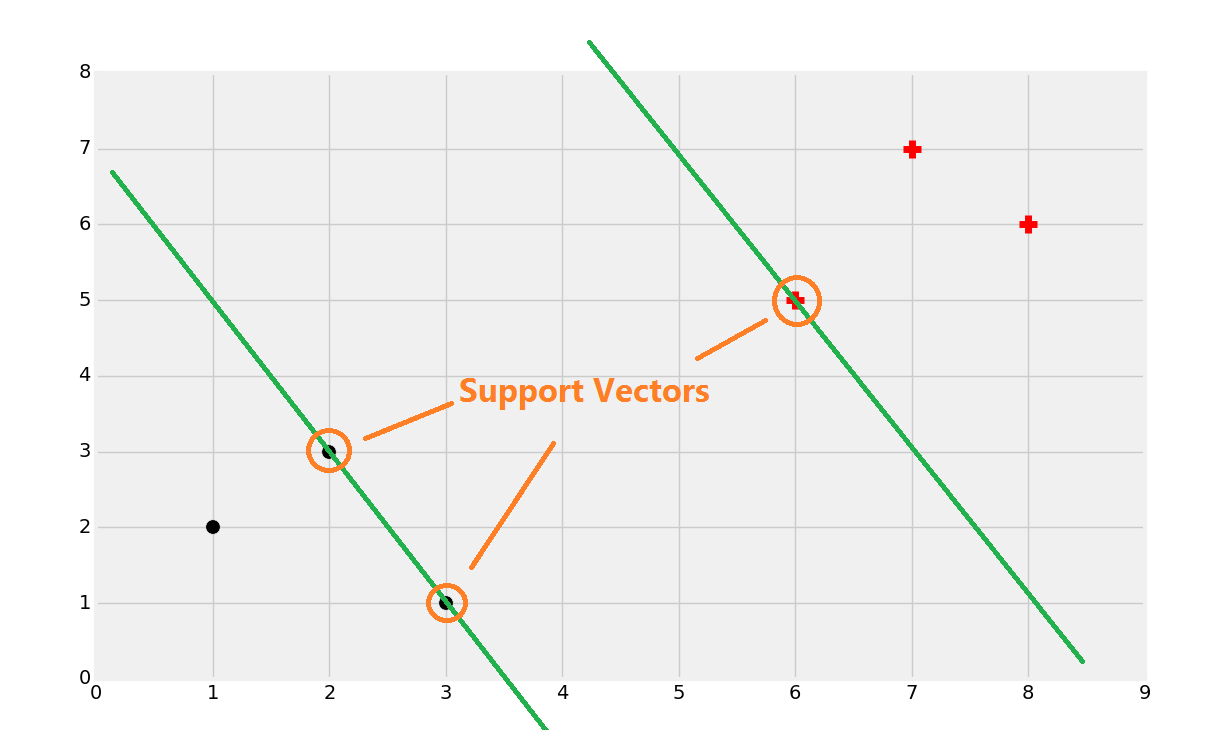
\includegraphics[width=0.8\textwidth]{images/svm-support-vectors.png}
\caption{\label{fig:svm-support-vectors} Shows the support vectors for this SVM classification problem.}
\end{figure}

\begin{figure}
\centering
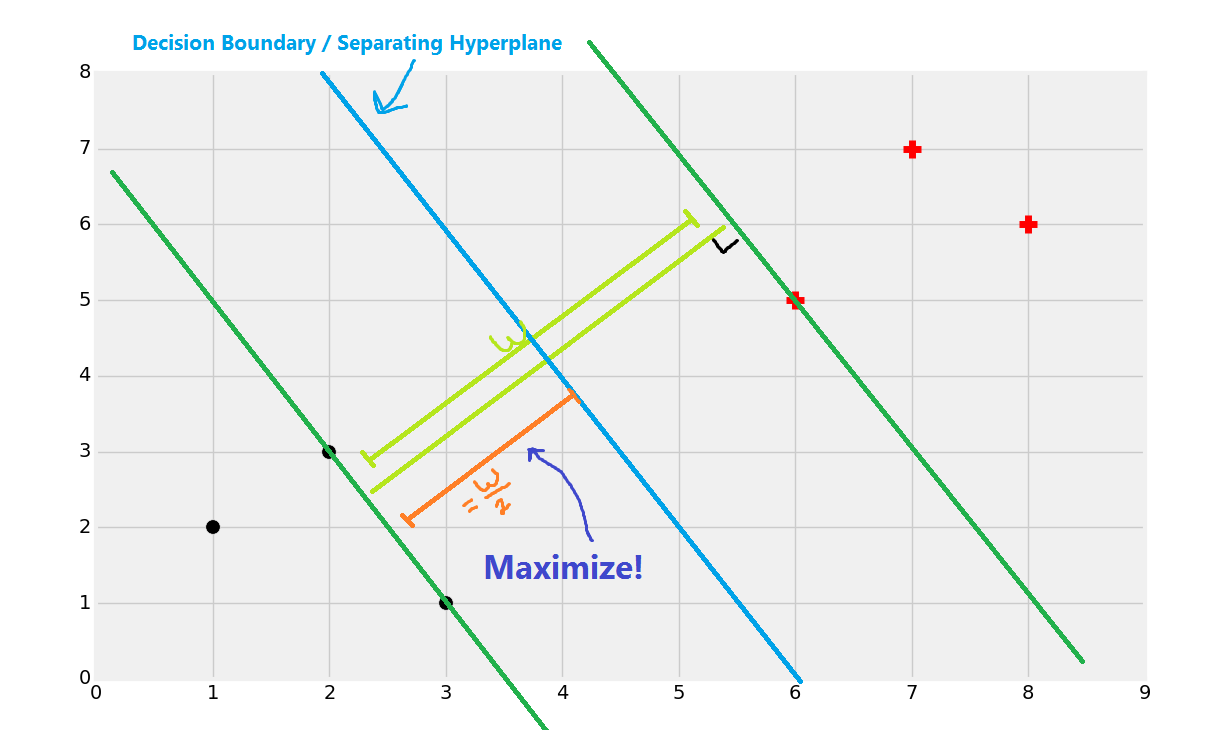
\includegraphics[width=0.8\textwidth]{images/svm-decision-boundary.png}
\caption{\label{fig:svm-decision-boundary} Shows the decision boundary for this SVM classification problem.}
\end{figure}

\subsection{Kernels}\label{sub:kernel}
Kernels are similarity functions, which take two inputs and return a similarity using inner products. This allows us to translate our data to a plausibly infinite number of dimensions in order to find one that has linear separbility, without paying the processing costs to do it. The only requirement to use kernels is to confirm that every interaction with our featurespace is an inner product. The formulas used for SVMs are transformable to inner products, so that is nice. %TODO We won't go in much detail but one example is our function %TODO x.w +b invoegen. daar kan je x.w vervangen door z en dan heb je een inner product (zie kernels tutorial)
Kernels are also used in other machine learning algorithms than SVMs.

%TODO explain more elaboratly

\subsection{Soft Margin SVMs}
A soft margin SVM allows for some slack on the errors that we might get in the optimisation process (While the standard SVM, a hard-margin, does not allow this wiggle room for error). You can use soft margin SVMs when your data is not perfectly linearly separable, but is very close or when you have a strong over-fitment when using a hard-margin SVM. An over-fitment can be recognised by the number of points on your support vectors versus the number of points of that class. For example if 100$\%$ of the positive class' points are on the support vector, this signals a high chance of over-fitment.
\\\\

%TODO add this when you want to talk in more detail about SVMs
% To allow for this error slack we introduce $\xi$, so our optimisation calculation becomes $y_i (x_i \cdot w + b) \geq 1 - \xi$ where $\xi \geq 0$, for a hard-margin $\xi = 0$. Ofcourse we'd like to minimise slack and for that we first introduce another variable $C$. $C$ is a multiplier for the value of how much we want $\xi$ to affect the rest of the equation, the lower $C$, the less important $\xi$ is in relation to the magnitude of vector w. $C$ is 1 by default. Now our full equation that we want to minimise is $\dfrac{1}{2} \Vert \overline{w} \Vert ^2 + C \sum\limits_i \xi_i$.

\subsection{OVR and OVO}\label{sub:ovr_ovo}
OVR or \emph{One Verse Rest} seperates each group from the rest and generates decision boundaries for all of these. For example if you have three classes, 1, 2 and 3. Then OVR would compare 1 to (2 and 3), 2 to (1 and 3) and 3 to (1 and 2) and generate decision boundaries for all three options. The problem is that you will almost always have more negatives than positives, since you're maybe comparing one group to three others. This means every classification boundary is actually unbalanced.
\\\\
OVO or \emph{One Verse One} compares every one class to all others. Thus 1 to 2, 1 to 3, 2 to 1, 2 to 3, 3 to 1 and 3 to 2 deliver all seperate decision boundaries. This tends to result in more balance results.

\begin{figure}
\centering
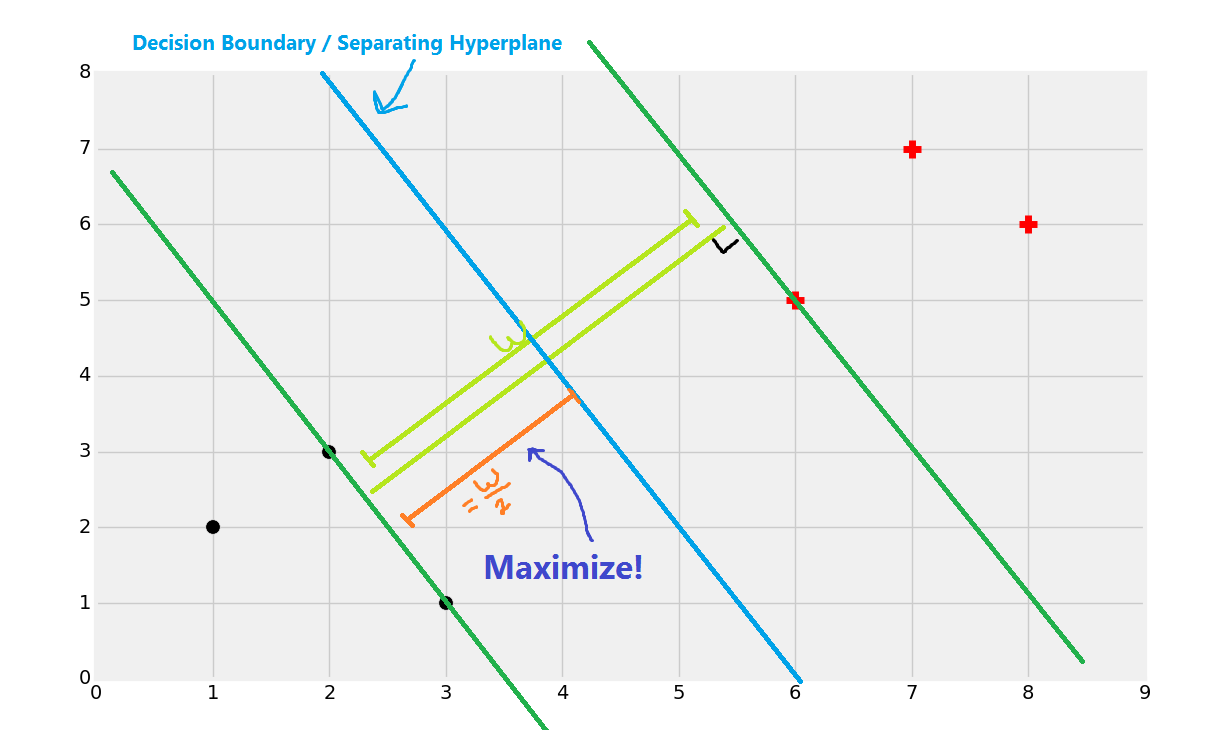
\includegraphics[width=0.8\textwidth]{images/svm-decision-boundary.png}
\caption{\label{fig:ovr} Shows the results of van OVR classification.}
\end{figure}

\subsection{Code examples}
Two code approaches have been made. The first approach uses the \emph{sklearn} kit, the approach can be found in appendix \ref{code:svm} and is very similar to appendix \ref{code:knn}. The second approach shows a more basic SVM which illustrates it's fundamentals. This code can help you understand the basic building blocks of the algorithm and let you see where it's pitfalls are. The code can be found in appendix \ref{code:msvm}. No detailed implementation of kernels, soft margin SVMs, OVO or OVR has been implemented.
